\chapter{Testing of the driver of LED7708}
\section{LED7708 Introduction}
The LED7708 has been specifically designed to supply several LEDs from a single low-voltage rail in
order to address TV and monitor backlights, medium- and large-size LCD panel backlights and
RGB/RGGB backlight applications. It has sixteen current generators rated at 40 V and a 4-wire serial
interface to control LED brightness. These channels can be put in parallel for higher output currents. A
selectable 12-bit or 16-bit gray-scale brightness control allows independent PWM on each channel. A
programmable on-chip dimming oscillator is provided to simplify external circuitry. The device has
dedicated pins to lock synchronize with other devices (master or slave) for noise reduction in multi-
device applications.\\
The LED7708 implements basic protection (OVP, OCP and thermal shutdown), as well as LED-array
protection. It can detect and manage open-LED and shorted-LED faults, and different fault
management options are available in order to cover most application needs. The board has been
designed as a demonstration of a solution for medium/large LCD panel backlight drivers, but is
suitable for any application involving several LEDs assembled in strings (e.g. advertisement panels,
signs, gaming, etc.).
\subsection{LED7708 read/write protocols}
Protocols for read and write LED7708 registers.
\subsubsection{Serial interface internal registers}
The internal registers are organized in control registers and brightness registers. Access to the desired
register is performed by encoding the destination address via a serial key on the bus (a serial key
consists of a certain number of clock pulses during the high-state of the LE signal). All the internal
registers are 16 bits wide. \\
\begin{table}[ht]
	\centering
	\scalebox{1}
	{
		\begin{tabular}{|K{5cm} | K{5cm}|}
			\toprule
			\rowcolor{Gray}
			\textbf{DCLK rsing edge with LE=1} & \textbf{operation} \\
			\hline
			1 & Data latch \\
			\hline
			2-3 & Global latch \\
			\hline 
			4-5 & Write CHSEL \\
			\hline
			6-7 & Read CHSTA \\
			\hline 
			8-9 & Write DEVCFG \\
			\hline
			10-11 & Read DEVCFG \\
			\hline
			11-12 & Write GSLAT \\
			\bottomrule
		\end{tabular}
	}
		\caption{Internal register operation encoding}
\end{table}
\subsection{LED7708 Linux device driver}
Below is the Linux kernel Architecture showing where all the basic components and their
functionality lies and showing where the LED7708 LDD fits in.
\begin{figure}[ht]
         \centering
         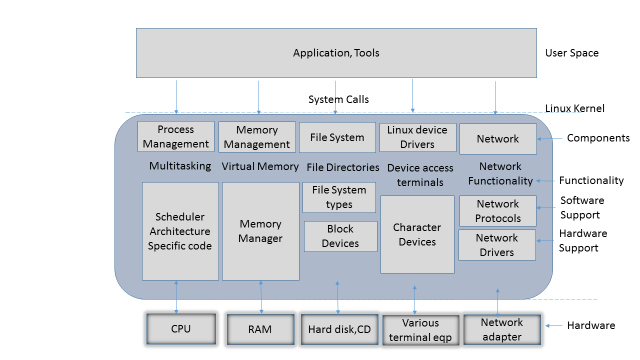
\includegraphics[scale=0.7]{images/kernel.png}
         \caption{Linux kernel architecture}
\end{figure}
\section{Interfacing of the LED7708 with RPI2 board}
\subsection{Hardware setup}
You will need the following items while working with LED7708 with Raspberry Pi 2\\
\begin{enumerate}
	\item \textbf{LED7708} Evaluation Board.
	\item A Connector or Jumper wires to connect LED7708 with the Rpi2 according to the connection
diagram shown in figure below.
	\item Standard HDMI cable for display along with a HDMI Monitor or also can alternatively work
	remotely on PC (Windows or Linux) using any remote terminal Application like Putty.
	\item RS232 FTDI hardware cable for taking serial Logs (Only for taking boot time debugging logs).
	\item Wireless/Wired Keyboard for running the test scripts if working directly (Not remotely) on the
	RPI2 board.
\end{enumerate}
\subsubsection{Hardware connection between LED7708 and RPI2 board}
\begin{figure}[ht]
         \centering
         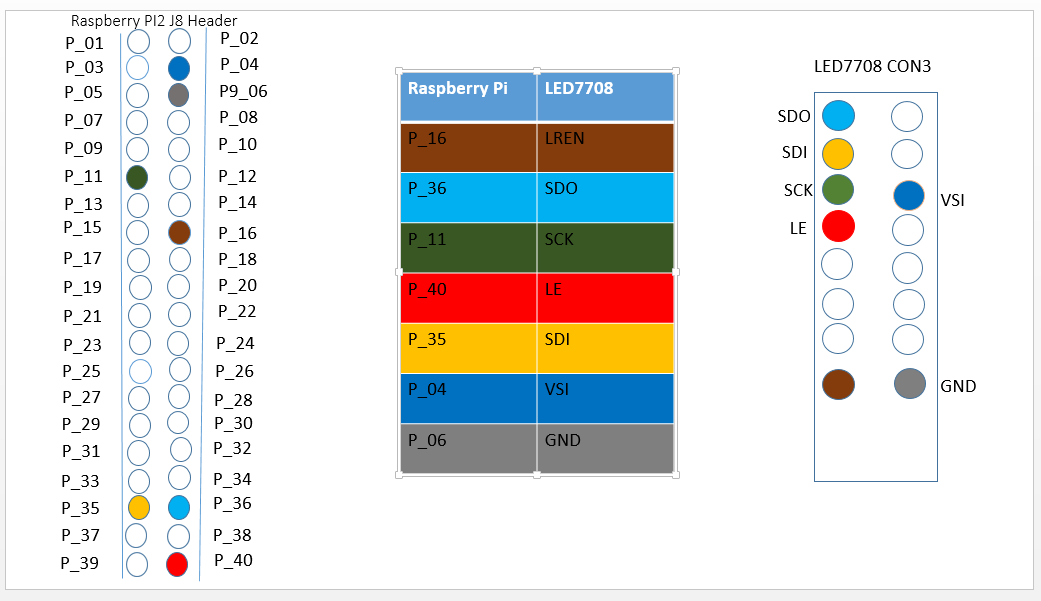
\includegraphics[scale=0.44]{images/raspberryled.png}
         \caption{Interfacing between LED board and RPI2}
\end{figure}
\subsubsection{Hardware Setup between RPI2 and LED7708 Eval board}
\begin{figure}[ht]
         \centering
         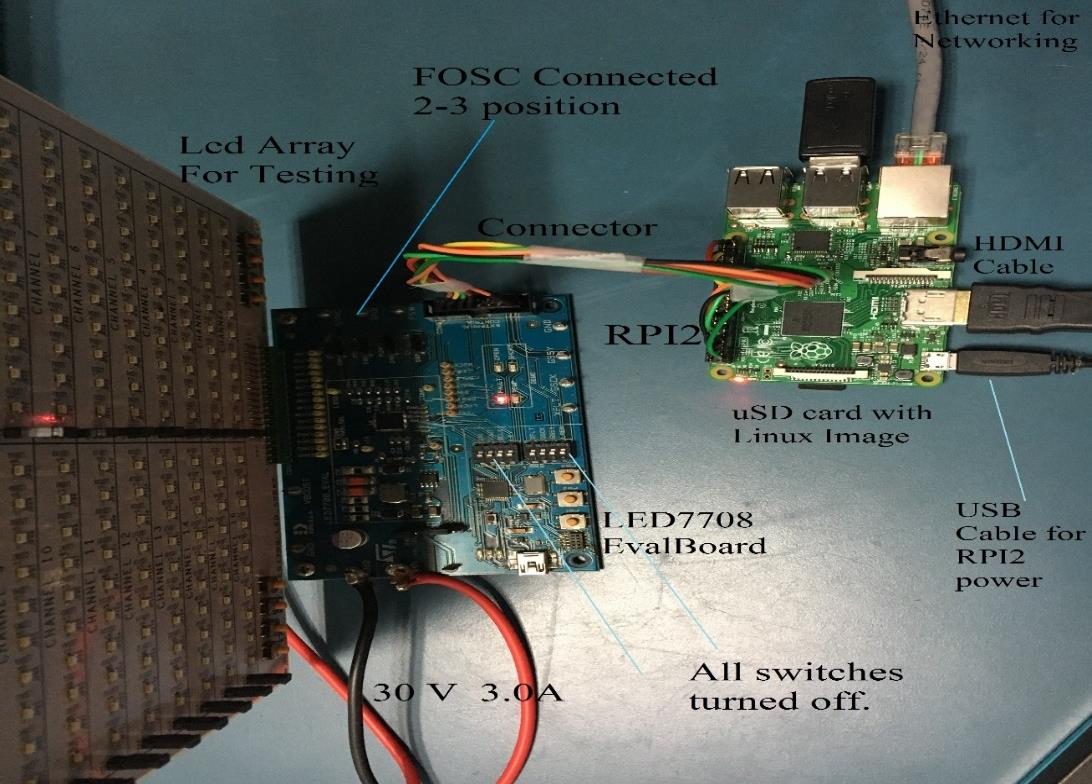
\includegraphics[scale=0.4]{images/raspberryledsetup.png}
         \caption{Hardware setup between LED7708 and RPI2 board}
\end{figure}
\subsection{Software setup}
For integrating the kernel driver with the Raspberry pi we have to bring up the RPI2 with the
appropriate Linux kernel. Please follow the below steps to prepare the RPI2 with Kernel 4.4.23
version.
\begin{enumerate}
	\item Download the kernel source
	Create a directory to store the Raspberry related files (e.g. /home/$<$my pc$>$/rpi2) and run the following
	command in that directory.\\
	git clone https://github.com/raspberrypi/linux.git \\
	if you want to branch to any other kernel run the below command .e.g below command will clone
	4.8.y branch. To see the available branches you can do git branch -a \\
	git checkout -b rpi-4.8.y --track origin/rpi-4.8.y
	\item Download the tool chain
	Tool chain will be required to build/compile the boot loader and the kernel sources.
	Download Raspberry PI cross-compilers by running the following command on your build
	machine.\\
	git clone https://github.com/raspberrypi/tools\\
	\item Configuring the kernel \\
	cd linux\\
	KERNEL=kernel7\\
	make ARCH=arm CROSS\_COMPILE=arm-linux-gnueabihf- bcm2709$_$defconfig
	\item Building the kernel
	Now it's time to build the kernel (image) and modules and .dtbs. Run this command in your terminal
	to build the kernel.\\
	make ARCH=arm CROSS\_COMPILE=arm-linux-gnueabihf- zImage modules dtbs
	\item Flashing the kernel on a new SD card
	Before that if you are using the new SD card you have to flash the NOOB or Raspbian image on it first
	and then follow the below steps.
	\begin{itemize}
		\item Download Raspbian image directly.
		using a computer with an SD card reader, visit the official Raspberry Pi Downloads page.
		\item Click on the Rasbian.
		\item Click on the Download ZIP button under ‘Raspbian Jessie (full desktop image)’, and select a folder
		to save it to.
		\item Extract the files from the zip.
		\item Visit \textbf{etcher.io} and download and install the Etcher SD card image utility.
		\item Run Etcher and select the Raspbian image you unzipped on your computer or laptop.
		\item Select the SD card drive. Note that the software may have already selected the right drive.
		\item Finally, click Burn to transfer Raspbian to the SD card. You'll see a progress bar that tells you how
		much is left to do. Once complete, the utility will automatically eject/unmount the SD card so it's safe
		to remove it from the computer.
	\end{itemize}
\end{enumerate}
\section{Adding Linux Device driver support in the Linux kernel}
Adding a LDD support in the Linux kernel means adding its source code in the Linux kernel. This
can be done either dynamically (building the driver as a module – out of the tree kernel
building) or by compiling the driver along with the kernel sources (in built driver). Also before
that Hardware (LED7708) specific parameters (like interface signals with the Raspberry PI)
needs to be defined to the kernel in the device tree of the platform in which LED7708 needs to
be interfaced.
\subsection{Adding Device tree bindings for LED7708 device driver}
Adding Device tree bindings for the Led7708 Linux driver.\\
In $<$path\_to\_kernel$>$/arch/arm/boot/dts/\\
nano bcm2709-rpi-2-b.dts\\
In this file make the entry for the led7708 board in the led class.\\
\subsection{Adding Linux driver in the kernel - Out of the tree}
Use the below Makefile to build the module.\\
\#MODULES := leds-st.o\\
ARCH := arm\\
CROSS\_COMPILE := arm-linux-gnueabihf-\\
obj-m := \$(MODULES)\\
OUTDIR := /$<$path to built kernel$>$/linux/\\
MAKEARCH := \$(MAKE) ARCH=\$(ARCH) CROSS\_COMPILE=\$(CROSS\_COMPILE)\\
all: modules\\
modules:\\
\$(MAKEARCH) -C \$(OUTDIR) M=\${shell pwd} modules\\
clean:\\
\$(MAKEARCH) -C \$(OUTDIR) M=\${shell pwd} clean\\
\section{Insert the modules}
Modules can be inserted using the commands \\
insmod leds-st.ko\\
Once the module is inserted successfully you can see the sysfs being created in the led directory and there is the sixteen channels for the leds class which you can access
directly and build your application by accessing them.\\
Example wave forms for the below sequence of commads:\\
\begin{itemize}
	\item W(08,04,2130)
	\item W(08,04,8440)
	\item W(04,04,FFFF)
	\item W(08,04,2131)
	\item W(02,04,FFFF)
\end{itemize}
Running the following scripts give the below waveform.
\begin{figure}[ht]
         \centering
         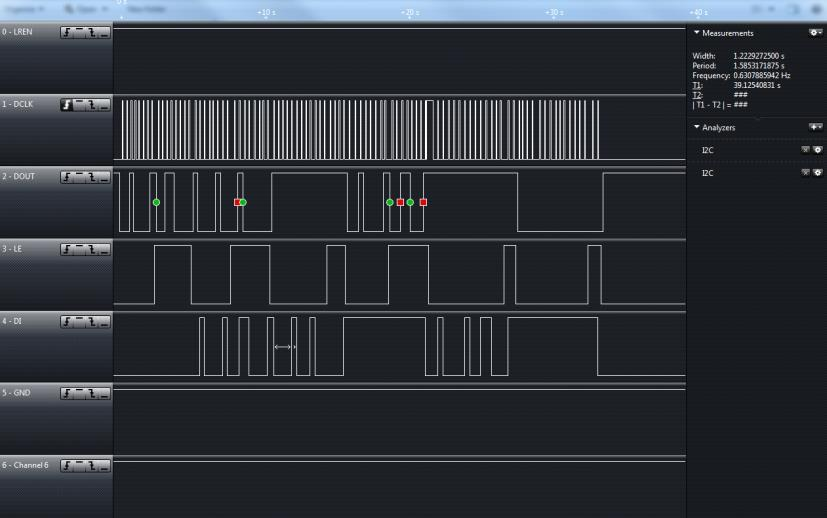
\includegraphics[scale=0.5]{images/waveform.png}
         \caption{Wave form for the example script}
\end{figure}








